\chapter{Introducci�n} 
\label{chap:intro}

\vspace{-0.2cm}

\lsection{Motivaci�n del proyecto}

Mi motivaci�n personal a la hora de embarcarme en este proyecto es la de crear un sistema heterog�neo, investigando as� campos como la programaci�n para dispositivos m�viles (en este caso, para Android) y las redes multimedia, materias en las que era m�s bien inexperto antes de comenzar con este trabajo. Por otra parte, mi experiencia en las pr�cticas de empresa que realic� en el proyecto de emprendimiento The Haptic Eye me animaron a llevar a cabo otro proyecto innovador, en tiempo real y que re�na tecnolog�as punteras en el estado del arte.


\lsection{Objetivos y enfoque}

% Esto quiz�s en el abstract mejor
A modo de s�ntesis, el objetivo inicial es desarrollar un sistema que proporcionara visi�n remota al
usuario mediante de un smartphone conectado, a trav�s de Internet, con un robot con dos c�maras
como si este �ltimo se tratase de un avatar.

El sistema consta, principalmente, de dos partes:
\begin{enumerate}  
\item Un Google Cardboard ~ y un tel�fono m�vil con Android desde el que ejecutar la
aplicaci�n. �sta estar� desarrollada utilizando la API de Google Cardboard [2]. En vez de
renderizar gr�ficos en 3D (Figura~\ref{fig:cardboard_3d}), simplemente se reproducir�n en tiempo real simult�neamente
dos v�deos (uno para cada ojo).


\begin{figure}[h]
	\centerline{
		\mbox{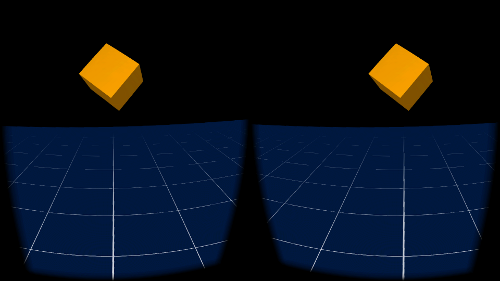
\includegraphics[width=3.00in]{images/cube2.png}}
	}
	\caption{\textbf{Ejemplo de aplicaci�n para Google Cardboard}. Utiliza OpenGL para renderizar los gr�ficos y los muestra para adaptarse a cada ojo.}
	\label{fig:cardboard_3d}
\end{figure}


\item Un peque�o robot con las siguientes caracter�sticas:
\end{enumerate}
\begin{itemize}
\item Dos videoc�maras.
\item Una estructura donde alojar estas dos c�maras.
\item Un motor que haga girar esta estructura sobre el eje vertical (Figura~\ref{fig:movimiento_cabeza})
\item Conectividad con la aplicaci�n a trav�s de Internet.
\end{itemize}

\begin{figure}[h]
	\centerline{
		\mbox{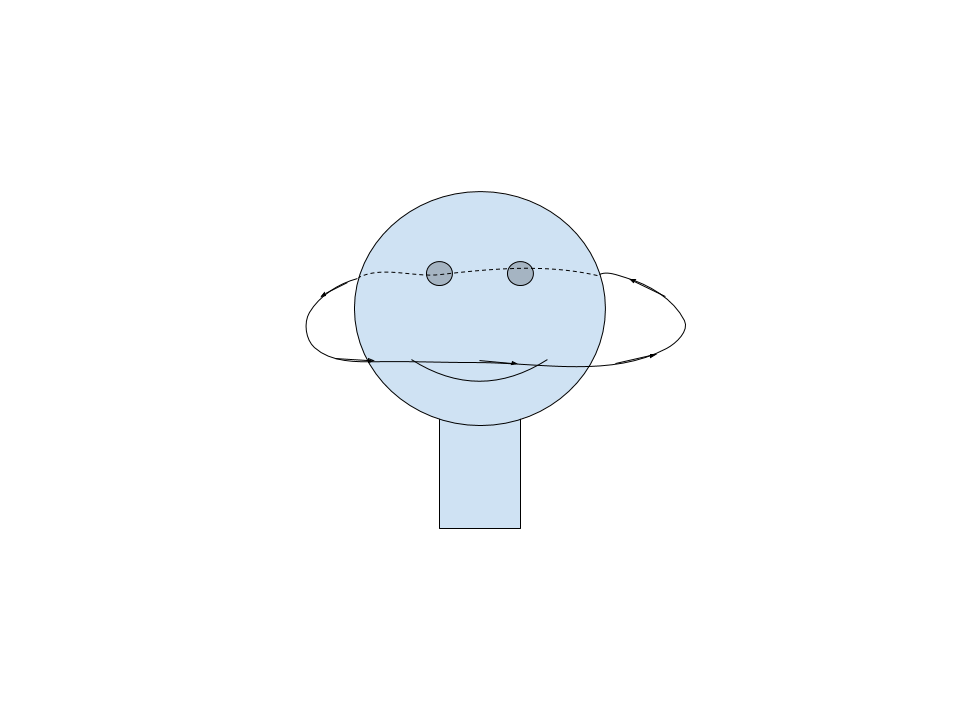
\includegraphics[width=3.00in]{images/movimiento_cabeza.png}}
	}
	\caption{\textbf{Movimiento de la cabeza} alrededor del eje vertical}
	\label{fig:movimiento_cabeza}
\end{figure}

\begin{figure}[h]
	\centerline{
		\mbox{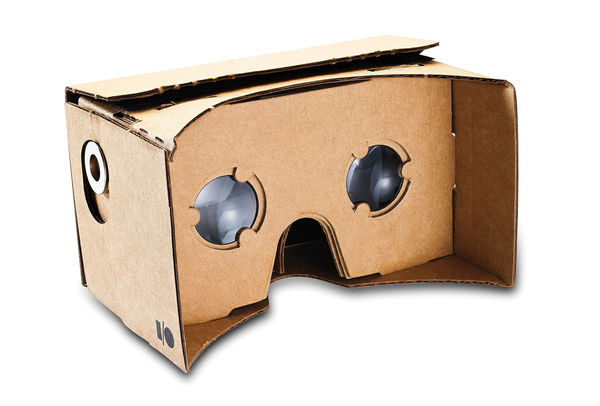
\includegraphics[width=3.00in]{images/googlecardboard.jpg}}
	}
	\caption{\textbf{Google Carbdoard}: las gafas de realidad virtual a partir de unas lentes, cart�n y un smartphone}
	\label{fig:googlecardboard}
\end{figure}

La aplicaci�n recibir� como entrada dos streams correspondientes a las c�maras de la
segunda parte y la posici�n en la que esta parte se encuentra (aunque en la pr�ctica esto �ltimo
quiz�s no haga falta). Como salida, enviar� la posici�n en la que se encuentra la cabeza del usuario
como comandos que el subsistema 2 procesar� y convertir� en instrucciones para los motores que
mueven su estructura.


\lsection{Metodolog�a y plan de trabajo}

\newpage \thispagestyle{empty} % P�gina vac�a 